% =================================================================================================
% =================================================================================================
%\appendix
% =================================================================================================
% =================================================================================================
\appendix
\appendixpage
\addappheadtotoc
\section{Pseudocódigo de software embebido}
\label{ap:pseudocodigo_software}

En este apéndice se reúnen los listados de pseudocódigo asociados a la arquitectura de software. Su objetivo es documentar el flujo lógico de operación sin interrumpir la descripción principal del diseño.

\subsection{Modelo de ejecución}

\begin{lstlisting}[
    style=pseudocodigo,language=Python, caption={Pseudocódigo del modelo de ejecución del sistema embebido.}, label={lst:modelo_ejecucion}]
    
def main():
    config = cargar_configuracion()

    colas_entrada = crear_colas_entrada(config.modulos)
    cola_estado = crear_cola_estado()

    modulos = instanciar_fsm(config.modulos, colas_entrada, cola_estado)

    router = crear_router()
    router.registrar_modulos(modulos, colas_entrada, cola_estado)

    scheduler = crear_scheduler(config.tareas, router)

    iniciar_procesos(modulos)
    scheduler.iniciar()

    emitir_senal_global(SIG_INIT, modulos)

    while sistema_activo():
        mensajes = leer_mensajes_estado(cola_estado)

        for mensaje in mensajes:
            router.procesar(mensaje)
            actualizar_estado_global(mensaje)
            persistir_evento(mensaje)

        scheduler.ejecutar_tareas_pendientes()

    emitir_senal_global(SIG_DEINIT, modulos)
    scheduler.detener()
    esperar_cierre_procesos(modulos)
    registrar_cierre_ordenado()
\end{lstlisting}

\subsection{Ciclo de vida de bajo nivel}

\begin{lstlisting}[style=pseudocodigo, caption={Pseudocódigo del ciclo de vida de un módulo de bajo nivel.}, label={lst:ciclo_vida_ll}]
init(configuracion):
    validar dependencias de software
    cerrar recursos previos si existen
    cargar parametros de configuracion
    resolver candidatos de transporte
    marcar modulo como inicializado
    retornar resultado

open():
    verificar que el modulo este inicializado

    si el recurso ya esta abierto:
        retornar OK

    intentar abrir el transporte configurado

    si no hay transporte forzado:
        probar candidatos disponibles

    si se abre correctamente:
        marcar recurso como abierto
        retornar OK

    registrar error
    retornar ERROR

full_test():
    construir reporte diagnostico
    recordar estado original del recurso

    si el recurso no esta abierto:
        abrir recurso temporalmente

    verificar presencia o comunicacion con el dispositivo
    recolectar informacion diagnostica disponible

    restaurar estado original del recurso

    retornar resultado y reporte

close():
    si el recurso esta abierto:
        cerrar transporte o recurso operativo

    marcar recurso como cerrado
    retornar resultado

deinit():
    cerrar recurso operativo
    limpiar transporte, candidatos y configuracion temporal
    marcar modulo como no inicializado
    retornar resultado
\end{lstlisting}

\subsection{Ciclo de operación de FSM}

\begin{lstlisting}[style=pseudocodigo, caption={Pseudocódigo del ciclo de operación de una Máquina de Estados Finitos.}, label={lst:ciclo_fsm}]
handle_message(mensaje):
    si estado == DISABLE:
        si mensaje == SIG_INIT:
            cambiar_estado(INIT)
        retornar

    si mensaje == SIG_DEINIT:
        cambiar_estado(DISABLE)
        retornar

    si mensaje == SIG_TEST:
        cambiar_estado(TEST)
        retornar

    si mensaje == SIG_ACQUIRE o mensaje == SIG_TIMEOUT:
        guardar_parametros_pendientes(mensaje)
        cambiar_estado(ACQUIRE)
        retornar


update():
    si no se ingreso a un nuevo estado:
        retornar

    marcar_entrada_procesada()

    si estado == INIT:
        resultado = ll.init()

        emitir_resultado_estado(resultado)

        si resultado == OK:
            cambiar_estado(TEST)
        si no:
            cambiar_estado(ERROR)

    si estado == TEST:
        resultado, detalles = ll.full_test()

        emitir_resultado_accion("test", resultado, detalles)

        si resultado == OK:
            cambiar_estado(IDLE)
        si no:
            cambiar_estado(ERROR)

    si estado == IDLE:
        esperar_eventos()

    si estado == ACQUIRE:
        resultado, datos = ejecutar_accion_principal(parametros_pendientes)

        emitir_resultado_accion("acquire", resultado, datos)

        si resultado == OK:
            cambiar_estado(IDLE)
        si no:
            cambiar_estado(ERROR)

    si estado == DISABLE:
        ll.deinit()

    si estado == ERROR:
        registrar_condicion_de_error()
        ll.deinit()
\end{lstlisting}

\subsection{Coordinación central}

\begin{lstlisting}[style=pseudocodigo, caption={Pseudocódigo de la coordinación central del sistema.}, label={lst:coordinacion_central}]
main():
    configuracion = cargar_configuracion()

    modulos = instanciar_modulos(configuracion)
    colas_entrada = crear_colas_de_entrada(modulos)
    cola_estado = crear_cola_de_estado()

    router = crear_enrutador_de_eventos()
    router.registrar_modulos(modulos, colas_entrada, cola_estado)

    scheduler = crear_planificador(configuracion.tareas, router)

    iniciar_procesos(modulos)
    scheduler.iniciar()

    enviar_senal_global(SIG_INIT, modulos)

    mientras sistema_activo():
        mensajes = leer_mensajes(cola_estado)

        para cada mensaje en mensajes:
            router.procesar(mensaje)
            actualizar_estado_global(mensaje)
            persistir_evento(mensaje)

        scheduler.ejecutar_tareas_pendientes()

    enviar_senal_global(SIG_DEINIT, modulos)

    scheduler.detener()
    esperar_cierre_de_procesos(modulos)
    registrar_cierre_ordenado()
\end{lstlisting}

\subsection{Enrutador de eventos}

\begin{lstlisting}[style=pseudocodigo, caption={Pseudocódigo simplificado del enrutador de eventos.}, label={lst:router_eventos}]
route(origen, mensaje):
    si origen pertenece a modulos_de_sensores
       y mensaje == ACTION_RESULT:
        guardar_ultima_lectura_compacta(origen, mensaje)
        retornar SIN_RUTEO

    si origen == AudioProc
       y mensaje == ACTION_RESULT:

        si resultado(mensaje) != OK:
            conservar_transmision_iridium_planificada()
            retornar SIN_RUTEO

        si mensaje contiene salida_acustica:
            guardar_ultimo_resumen_acustico(mensaje)
            retornar SIN_RUTEO

    para cada regla en reglas_de_ruteo:
        si regla coincide con origen y tipo_de_mensaje:
            si condicion_de_regla(mensaje) es verdadera:
                mensaje_ruteado = construir_mensaje_destino(mensaje)
                enviar_a_cola(regla.destino, mensaje_ruteado)
                retornar RUTEADO

    registrar_que_no_hubo_regla_aplicable()
    retornar SIN_RUTEO
\end{lstlisting}

\subsection{Selección de empaquetado acústico}

\begin{lstlisting}[style=pseudocodigo, caption={Selección de empaquetado para productos acústicos.}, label={lst:seleccion_empaquetado_audio}]
seleccionar_empaquetado_audio(relative_band_power_db):
separar valores por canal
cuantizar cada valor en decimas_de_dB

si todos los canales pueden codificarse como delta:
    packing = DELTA_PREVIOUS_INT8
    message_type = tipo_delta_segun_cantidad_de_canales
    audio_payload = primer_valor_int16_y_deltas_int8_por_canal

si no:
    packing = ABS_INT16
    message_type = tipo_absoluto_segun_cantidad_de_canales
    audio_payload = valores_int16_por_canal

body = cabecera(message_type, timestamp) + audio_payload
crc = crc16_ccitt_false(body)

retornar body + crc

\end{lstlisting}

\clearpage

\section{Evidencia documental de telemetría satelital}
\label{ap:evidencia_telemetria_satelital}

En este apéndice se incorporan tres reportes PDF asociados a los ensayos de telemetría satelital. Los documentos corresponden a payloads Iridium SBD recibidos por la unidad con IMEI~300534063350070 y a la corrida consolidada de decodificación utilizada para verificar la compatibilidad de los mensajes con el protocolo vigente.

\subsection{Reporte de payload Iridium MOMSN 120}
\label{ap:reporte_sbd_momsn_120}

El reporte incluido a continuación documenta la decodificación del payload MOMSN~120 como mensaje \texttt{MSG\_SYSTEM\_STATUS}, con campos de batería, almacenamiento, tiempo de operación, banderas de estado y mapas de estado de módulos.

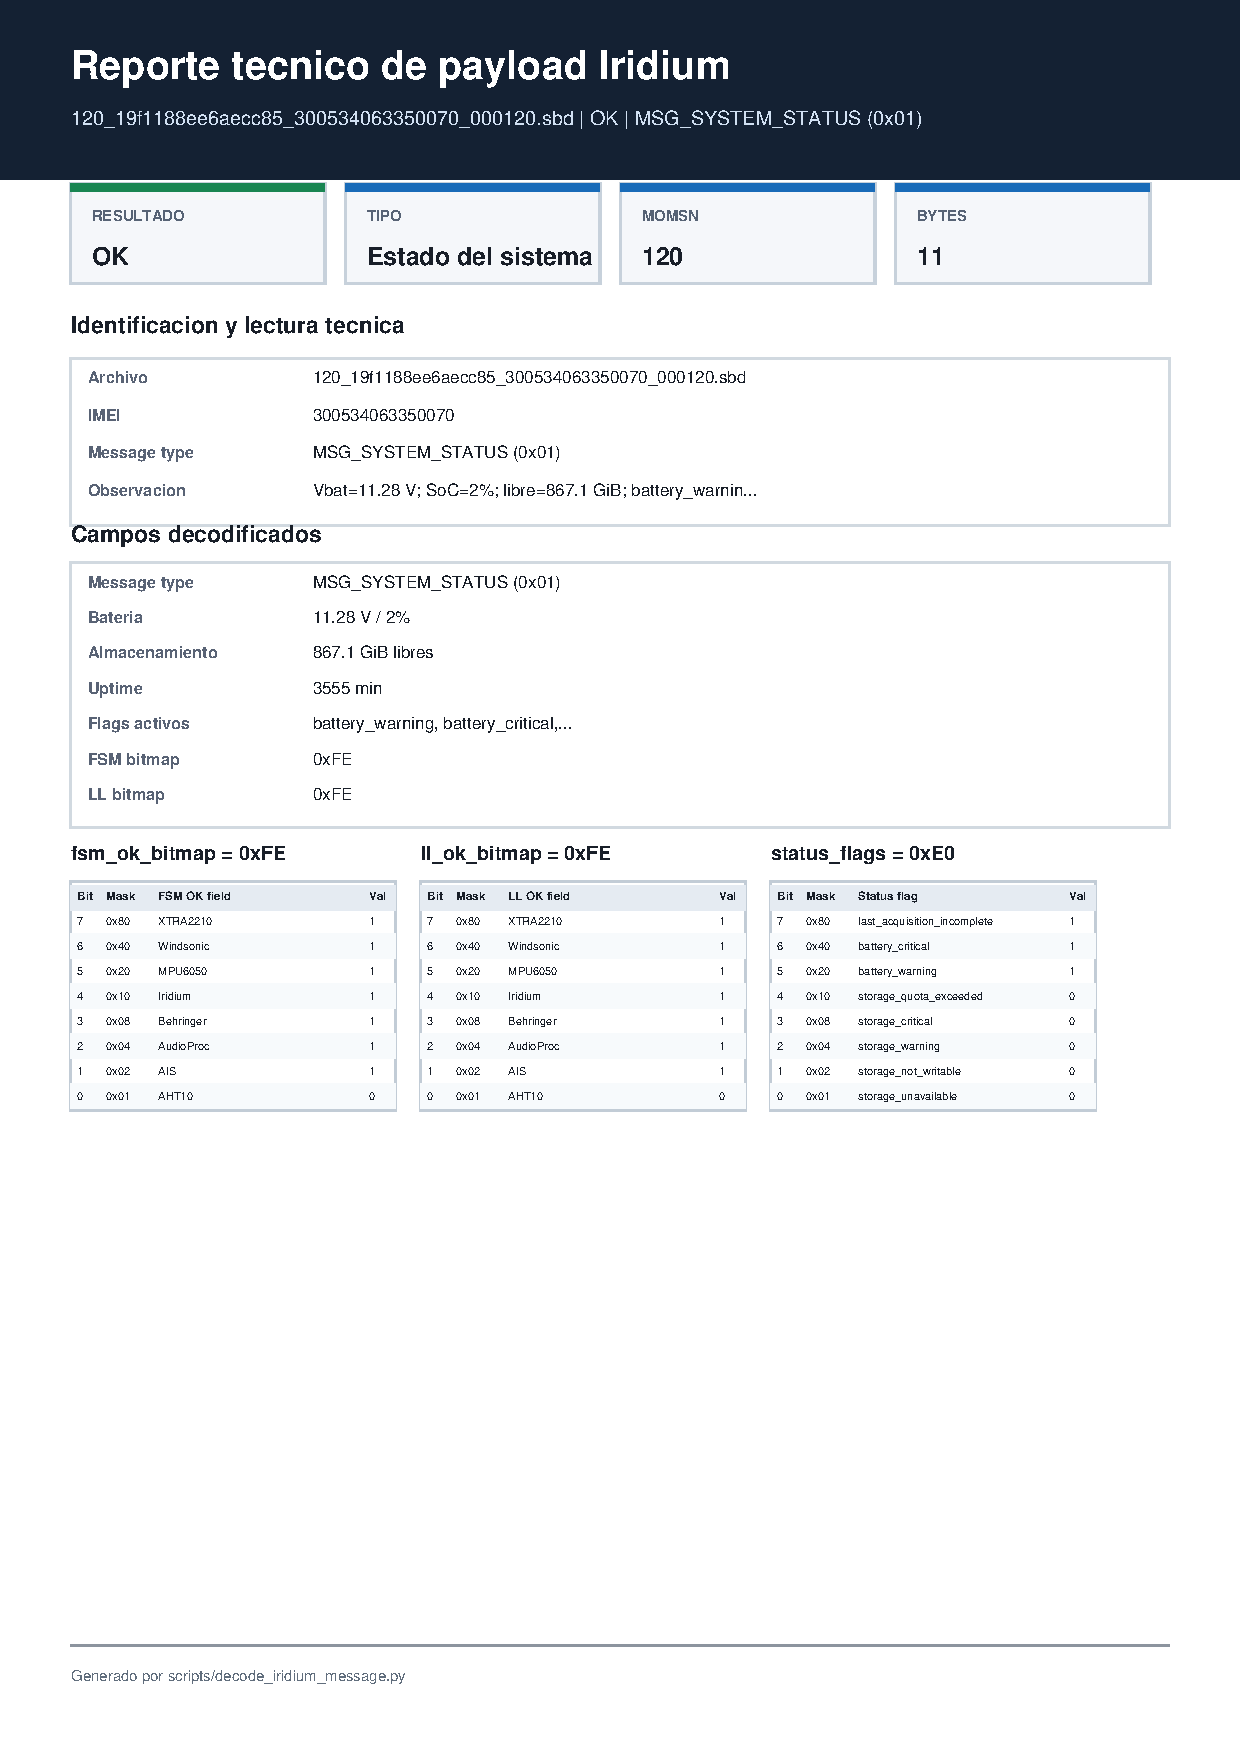
\includepdf[pages=-,scale=0.95,pagecommand={\thispagestyle{plain}}]{graficos/120_19f1188ee6aecc85_300534063350070_000120.pdf}

\clearpage

\subsection{Reporte de payload Iridium MOMSN 123}
\label{ap:reporte_sbd_momsn_123}

El reporte incluido a continuación documenta la decodificación del payload MOMSN~123 como mensaje \texttt{MSG\_AUDIO}, incluyendo cantidad de canales, cantidad de bandas, tipo de empaquetado, verificación CRC y valores de potencia relativa por banda.

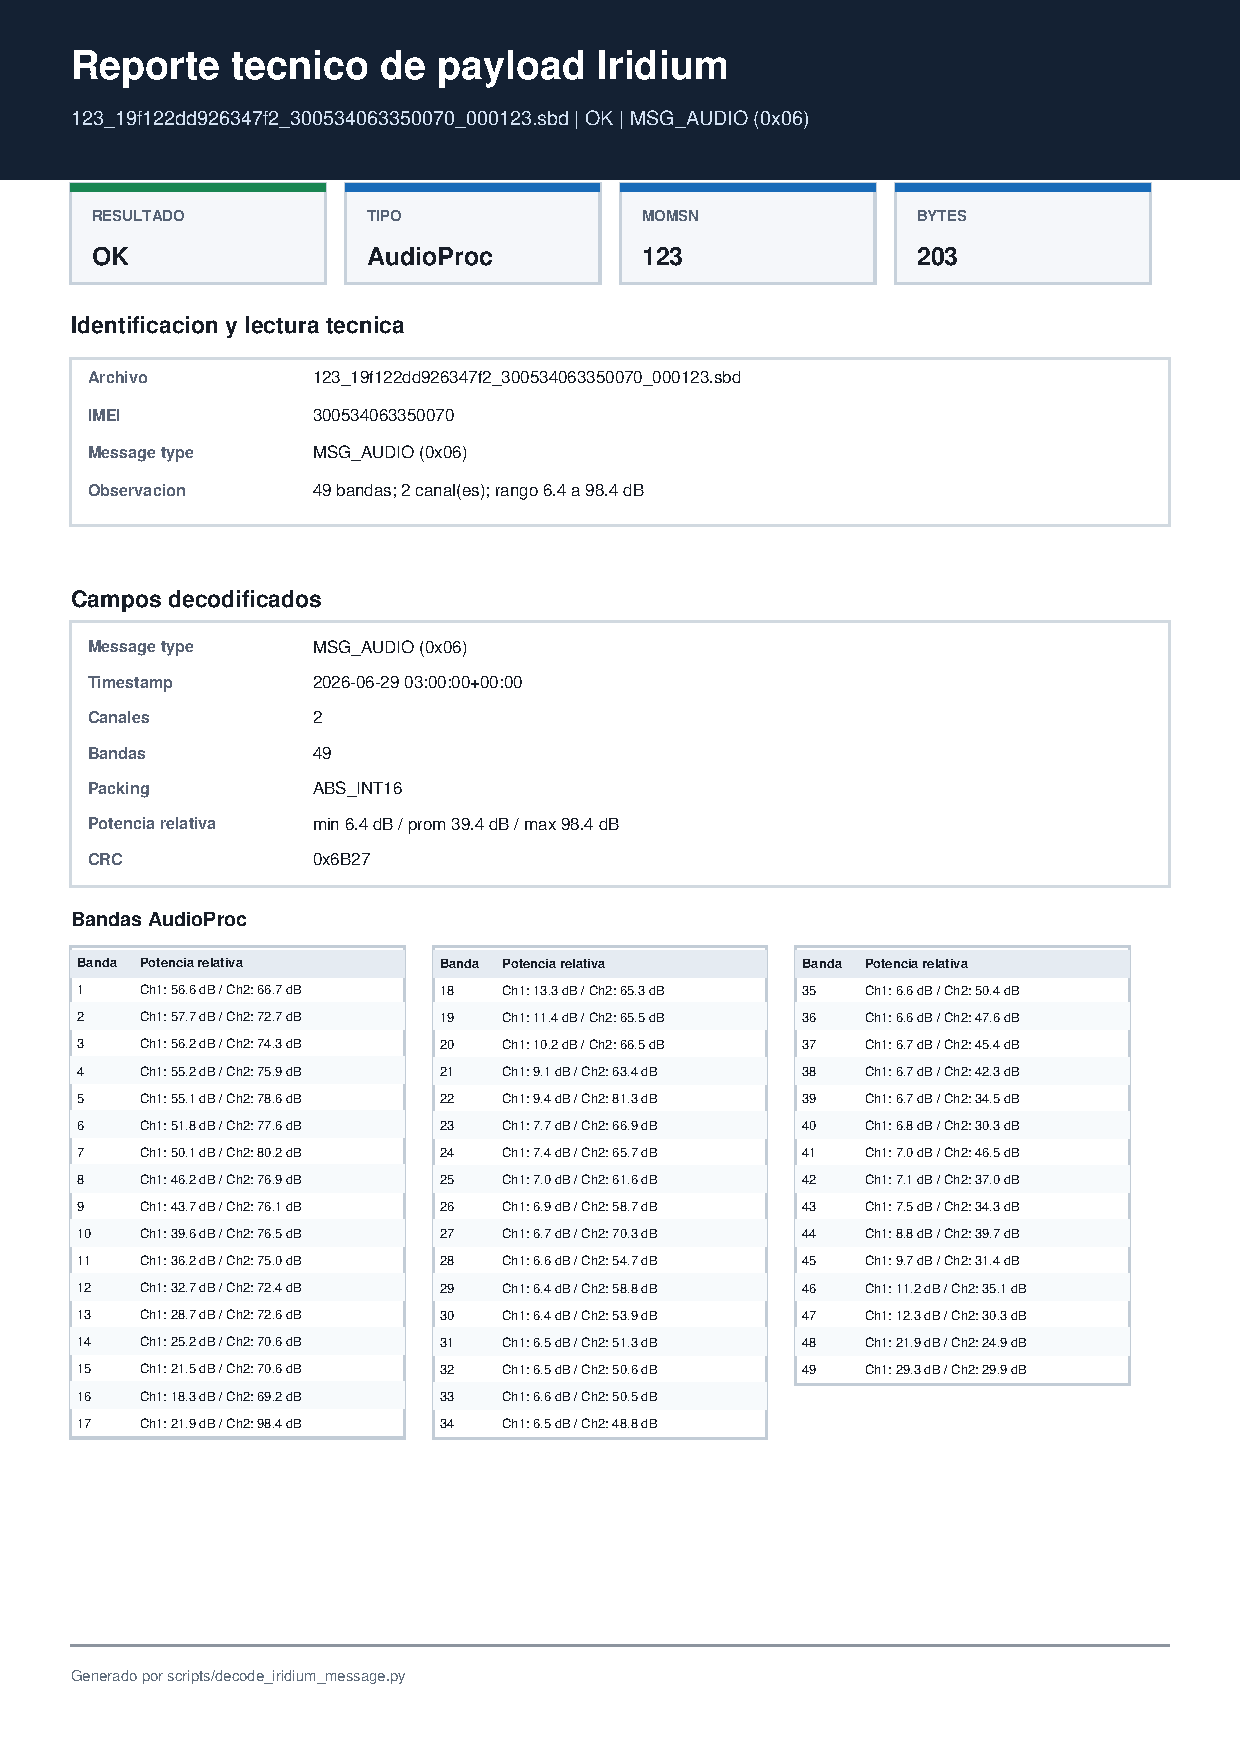
\includepdf[pages=-,scale=0.95,pagecommand={\thispagestyle{plain}}]{graficos/123_19f122dd926347f2_300534063350070_000123.pdf}

\clearpage

\subsection{Reporte consolidado de decodificación de payloads}
\label{ap:reporte_payloads_iridium}

El reporte incluido a continuación resume la corrida de decodificación aplicada al conjunto de payloads compatibles con el protocolo vigente. Este documento registra la cantidad total de archivos procesados, la ausencia de errores de decodificación, la distribución por tipo de mensaje y los rangos principales observados para los productos de AudioProc.

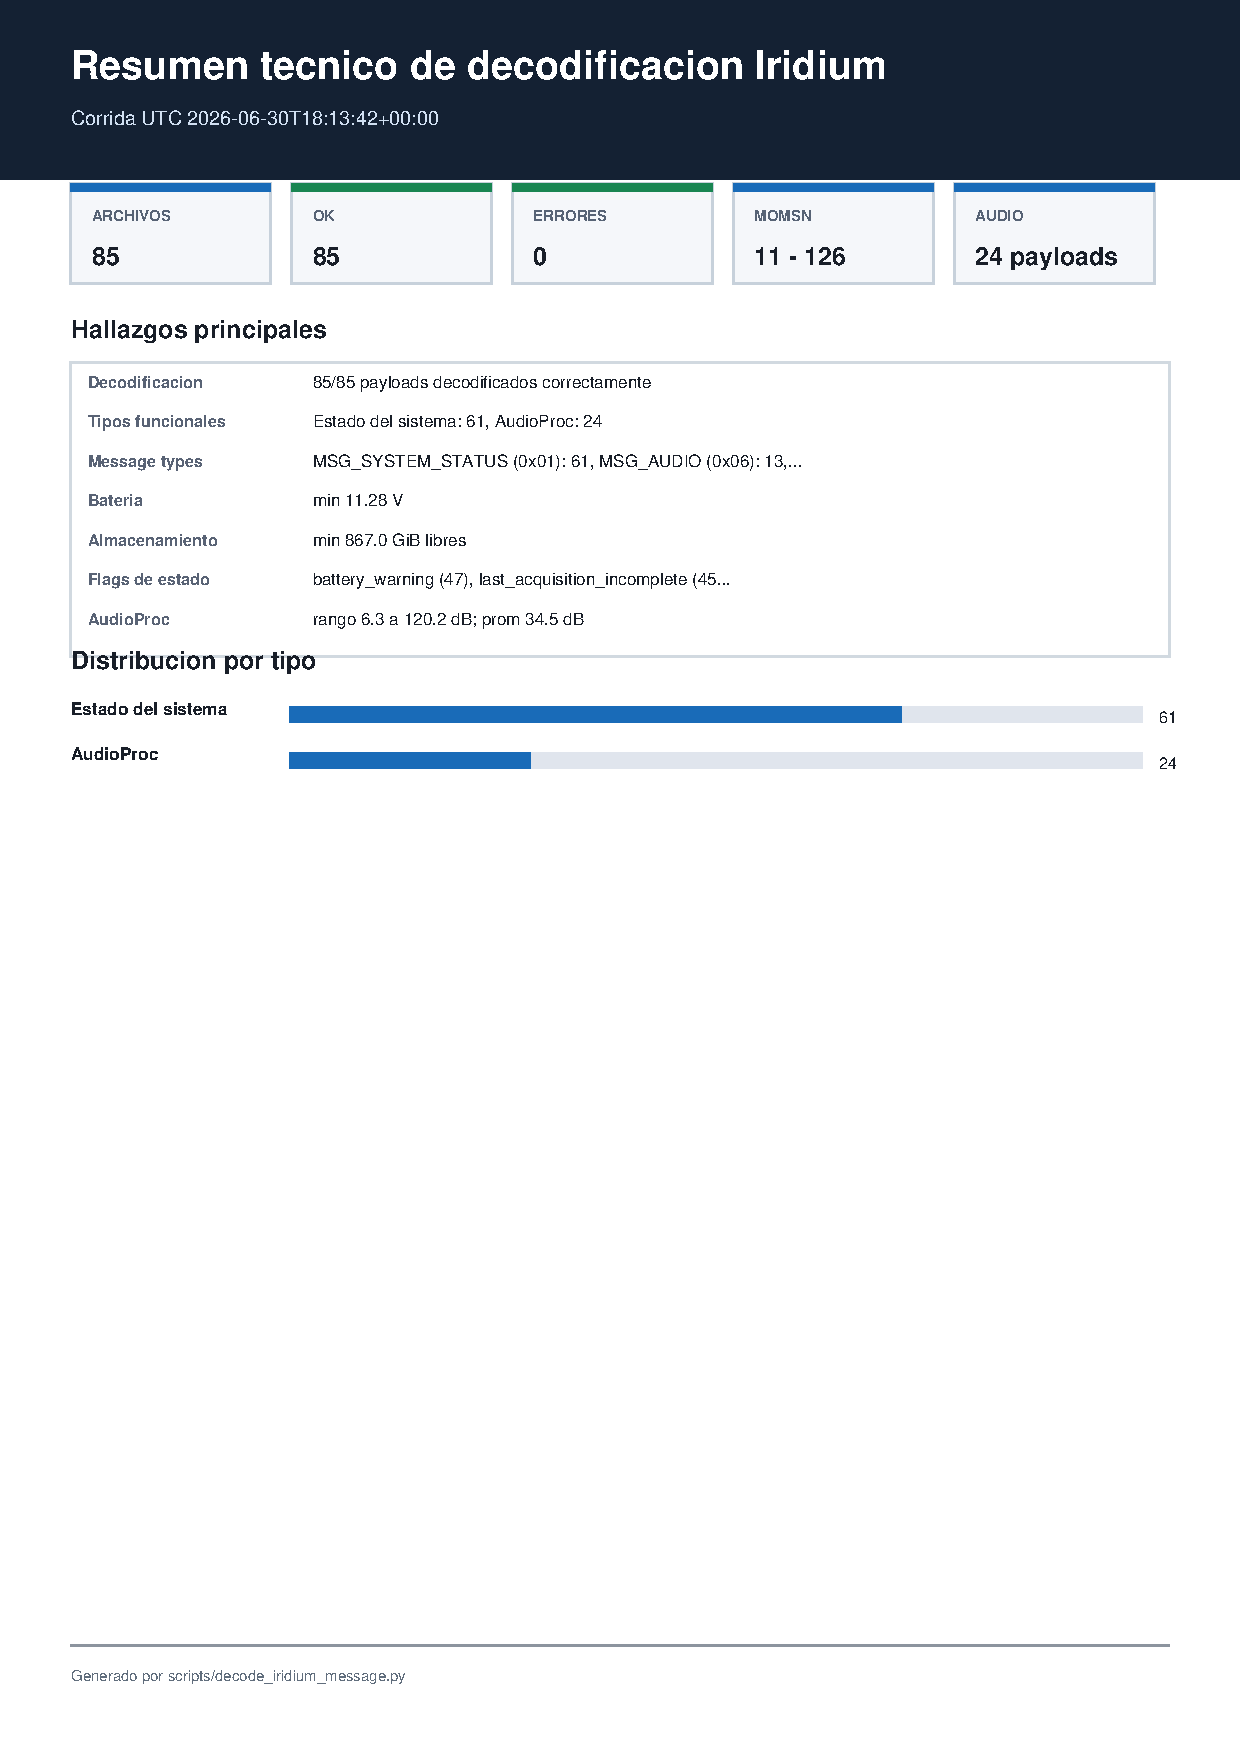
\includepdf[pages=-,scale=0.95,pagecommand={\thispagestyle{plain}}]{graficos/payloads_report.pdf}
